\section{Third Member}
This is the section dedicated to one of the team members, and it should be written individually . It can include a range of things; first subsection is a space for you to point out the strengths and weaknesses of the module, including complaints about the module coordinator Max Wilson. The second section should have a selfie image with Max! The last part of it is the most important one. You will need to write a paragraph about what you have learned in this module. You can write it in \textbf{Bold} if you want or you can use other fonts. 


\subsection{Comments about the module}

My strengths in this module are the concept of teamwork and achieving good structure when it comes to constructing graphs and figures, while working in a group while my weakness is that it sometimes takes me a while to figure out how to do I want.


\subsection{Selfie with Max}

\begin{figure}[h]
\caption{Selfie with Max}
\centering
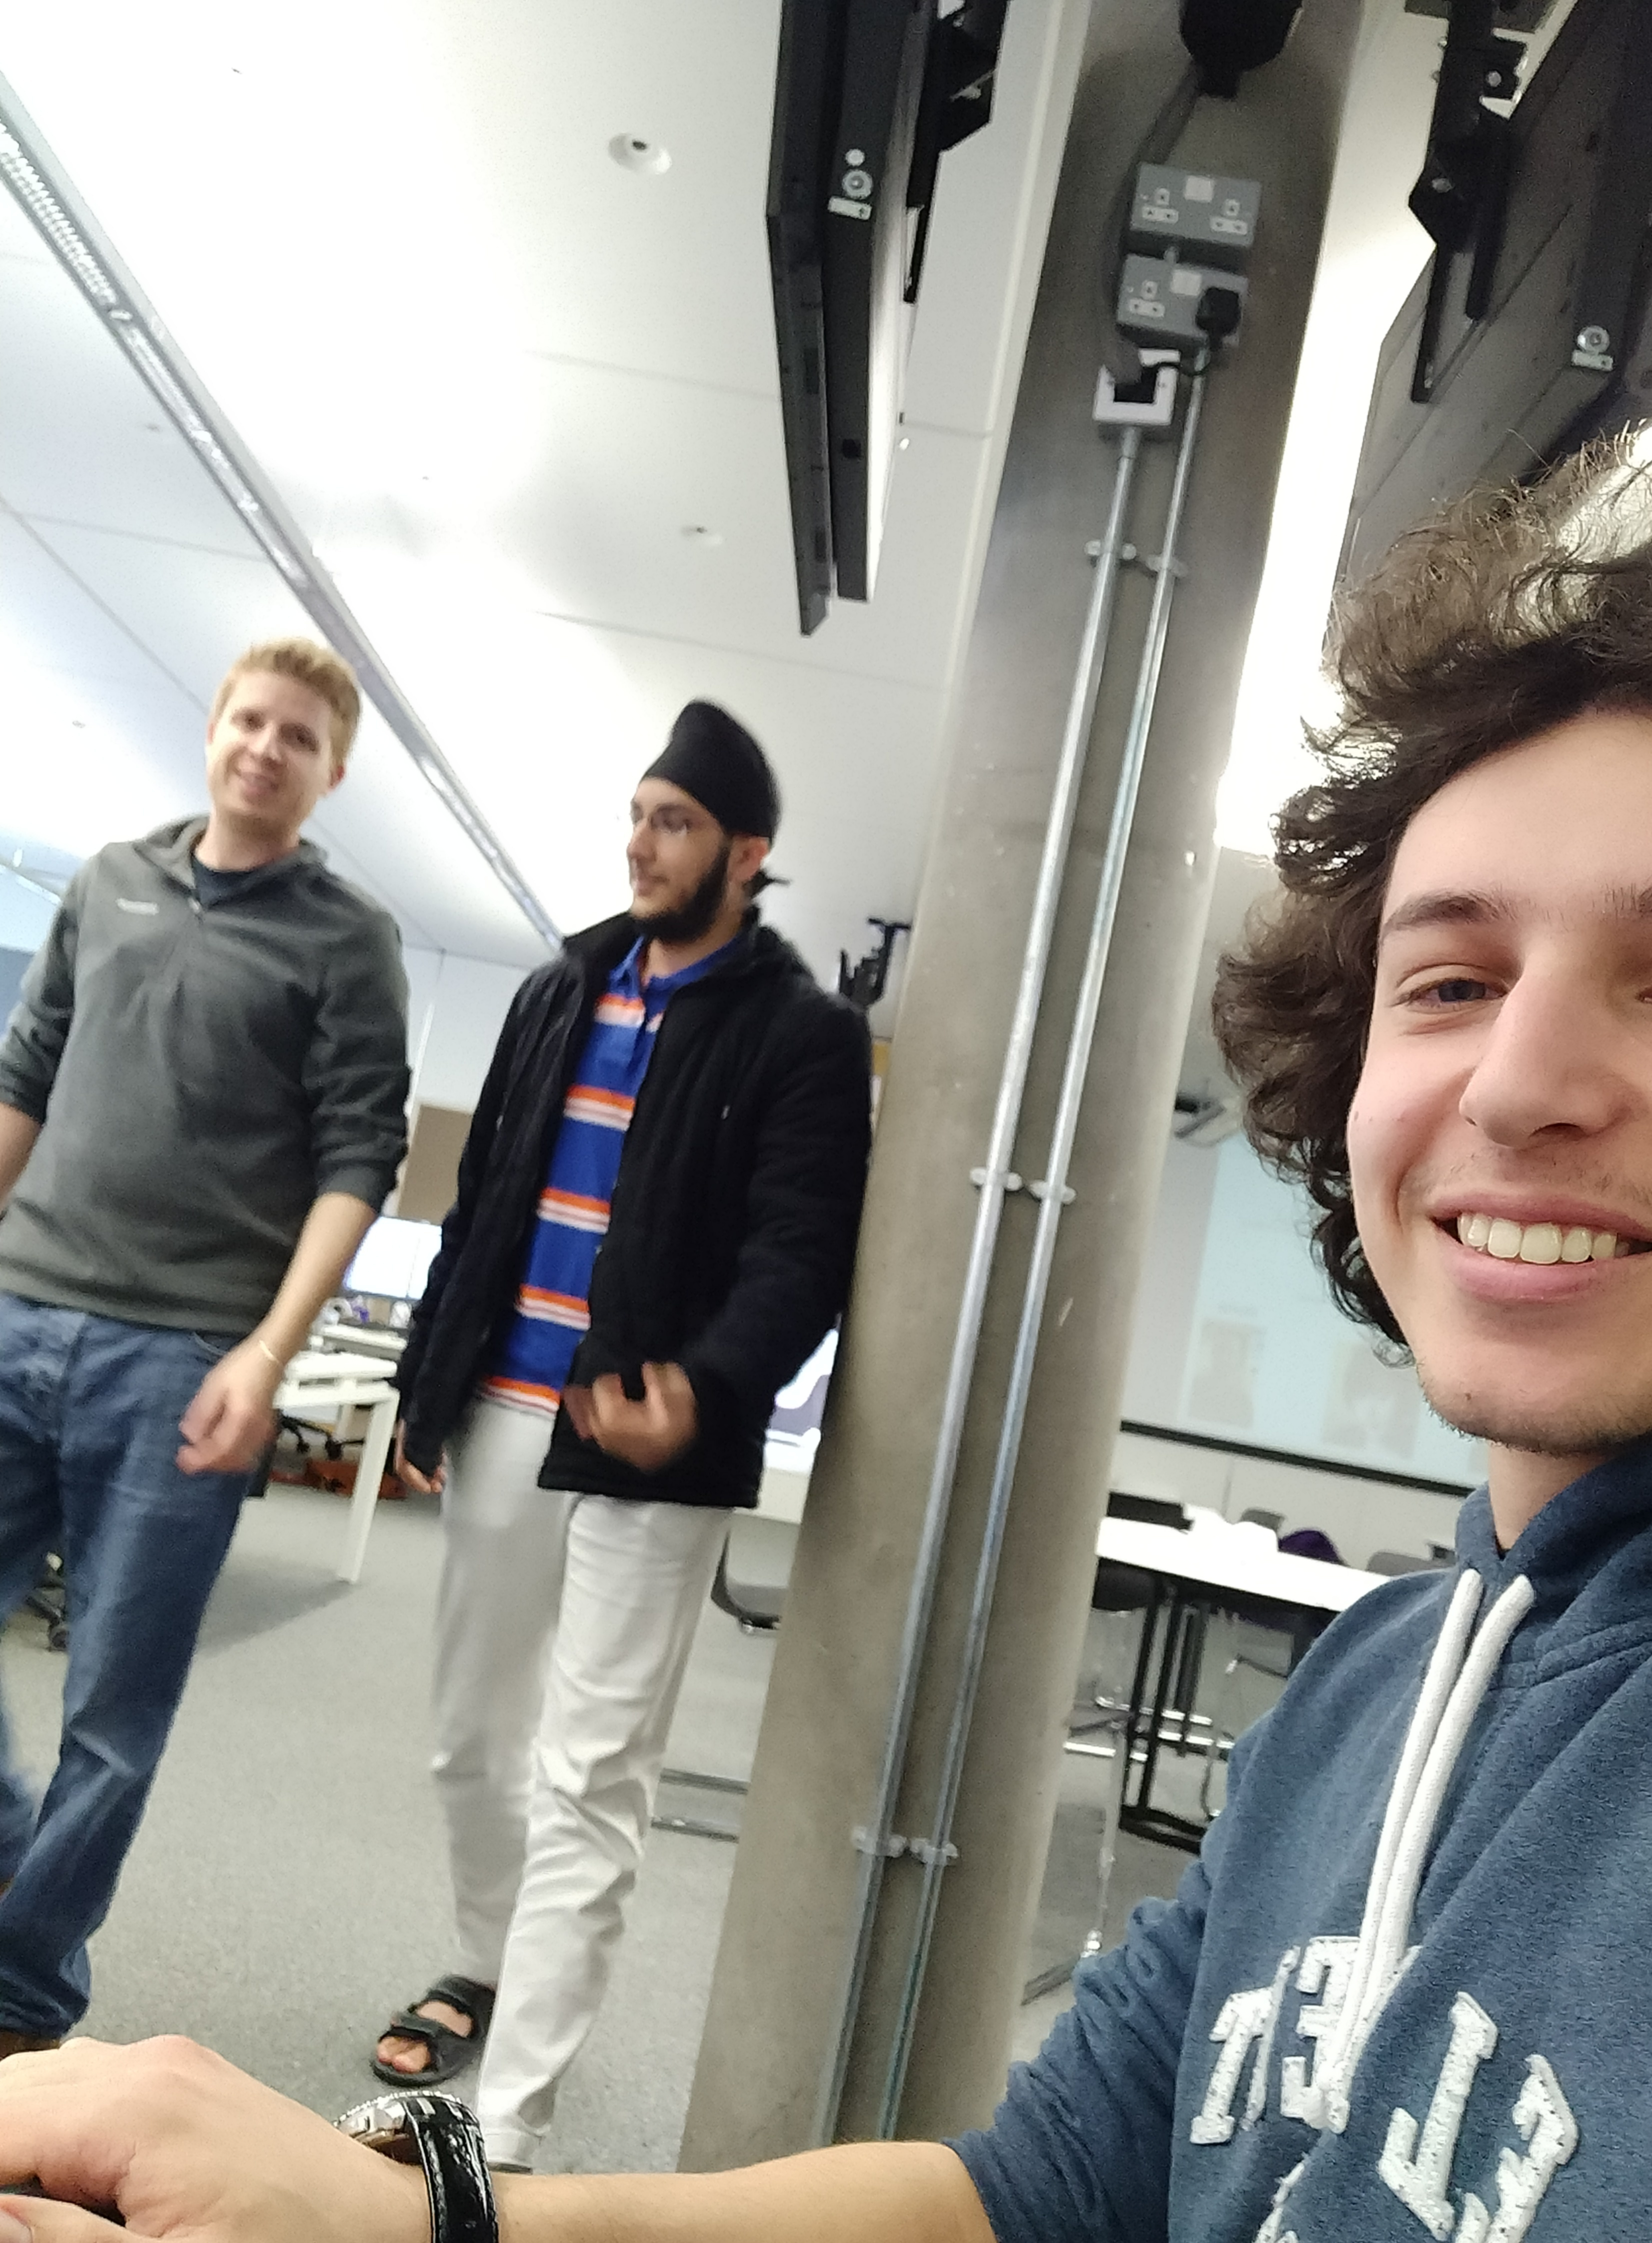
\includegraphics[width=0.5\textwidth]{selfie_with_Max.jpg}
\label{fig:selfie}
\end{figure}


\subsection{What I have learned in this module}

I have learned a lot about how a system should be designed, implemented and tested and how important that is.


